\chapter{Results}\label{sec:cap4}

This chapter presents the results obtained from the implemented models, including their performance metrics and comparisons. The models are evaluated based on their ability to detect anomalies in the discharge data and the lead time they provide before a disruption occurs.

\section{GitHub Organization}

This project uses git to handle different versions. As multiple software has been developed in this project, a GitHub Organization has been created in order to ease the cloning process.

The main repositories available on the organization are:

\begin{itemize}
    \item \textbf{Outlier orchestrator:} This repository contains the orchestrator explained at \autoref{sec:orchestrator}. 
    \item \textbf{py\_xgboost:} This repository contains the implementation of the XGBoost model \autocite{OutlierClassifierPy_xgboost2025}.
\end{itemize}

\section{Model Analysis and optimization}

This section provides an analysis of the models implemented in this project, focusing on their performance metrics and the optimization techniques applied to enhance their accuracy and efficiency. To do so, some discharges from the C24 campaign are selected for a deep analysis. These discharges are representative of different operational scenarios and include both normal and anomalous events. 

\subsection{XGBoost}

XGBoost implementation uses the features described in \autoref{subsubsec:xgboost}, which includes features from the current window and past windows as a tendency. This approach allows the model to have a better understanding of the discharge behavior over time, but also makes the model more rigid to changes in the discharge pattern. Additionally, model is trained with the C23 campaign and tested with the C24 campaign, which leads to a model that detects anomalies in the C24 campaign, but with some false positives because of the differences between the two campaigns, as explained in \autoref{apx:campaigns}. To reduce the false positives, orchestrator is configured to use a \textit{count threshold}, which means that more than one window must be labeled as anomalous in order to trigger an alert. 

Using the microservice approach, two XGBoost models are deployed, both with the same C23 training data, but while \texttt{xgboost\_2} uses a \textit{count threshold} of 2, \texttt{xgboost\_3} uses a \textit{count threshold} of 3. The automated predicts configuration is shown in \autoref{fig:xgboost-config}.

Increasing the \textit{count threshold} highly reduces the number of false positives, but also increases the lead time, as more windows must be labeled as anomalous before triggering an alert. With this settings, both models detect anomalies with any false negatives, but with some false positives, as explained in the next sections.

\begin{figure}[H]
    \centering
    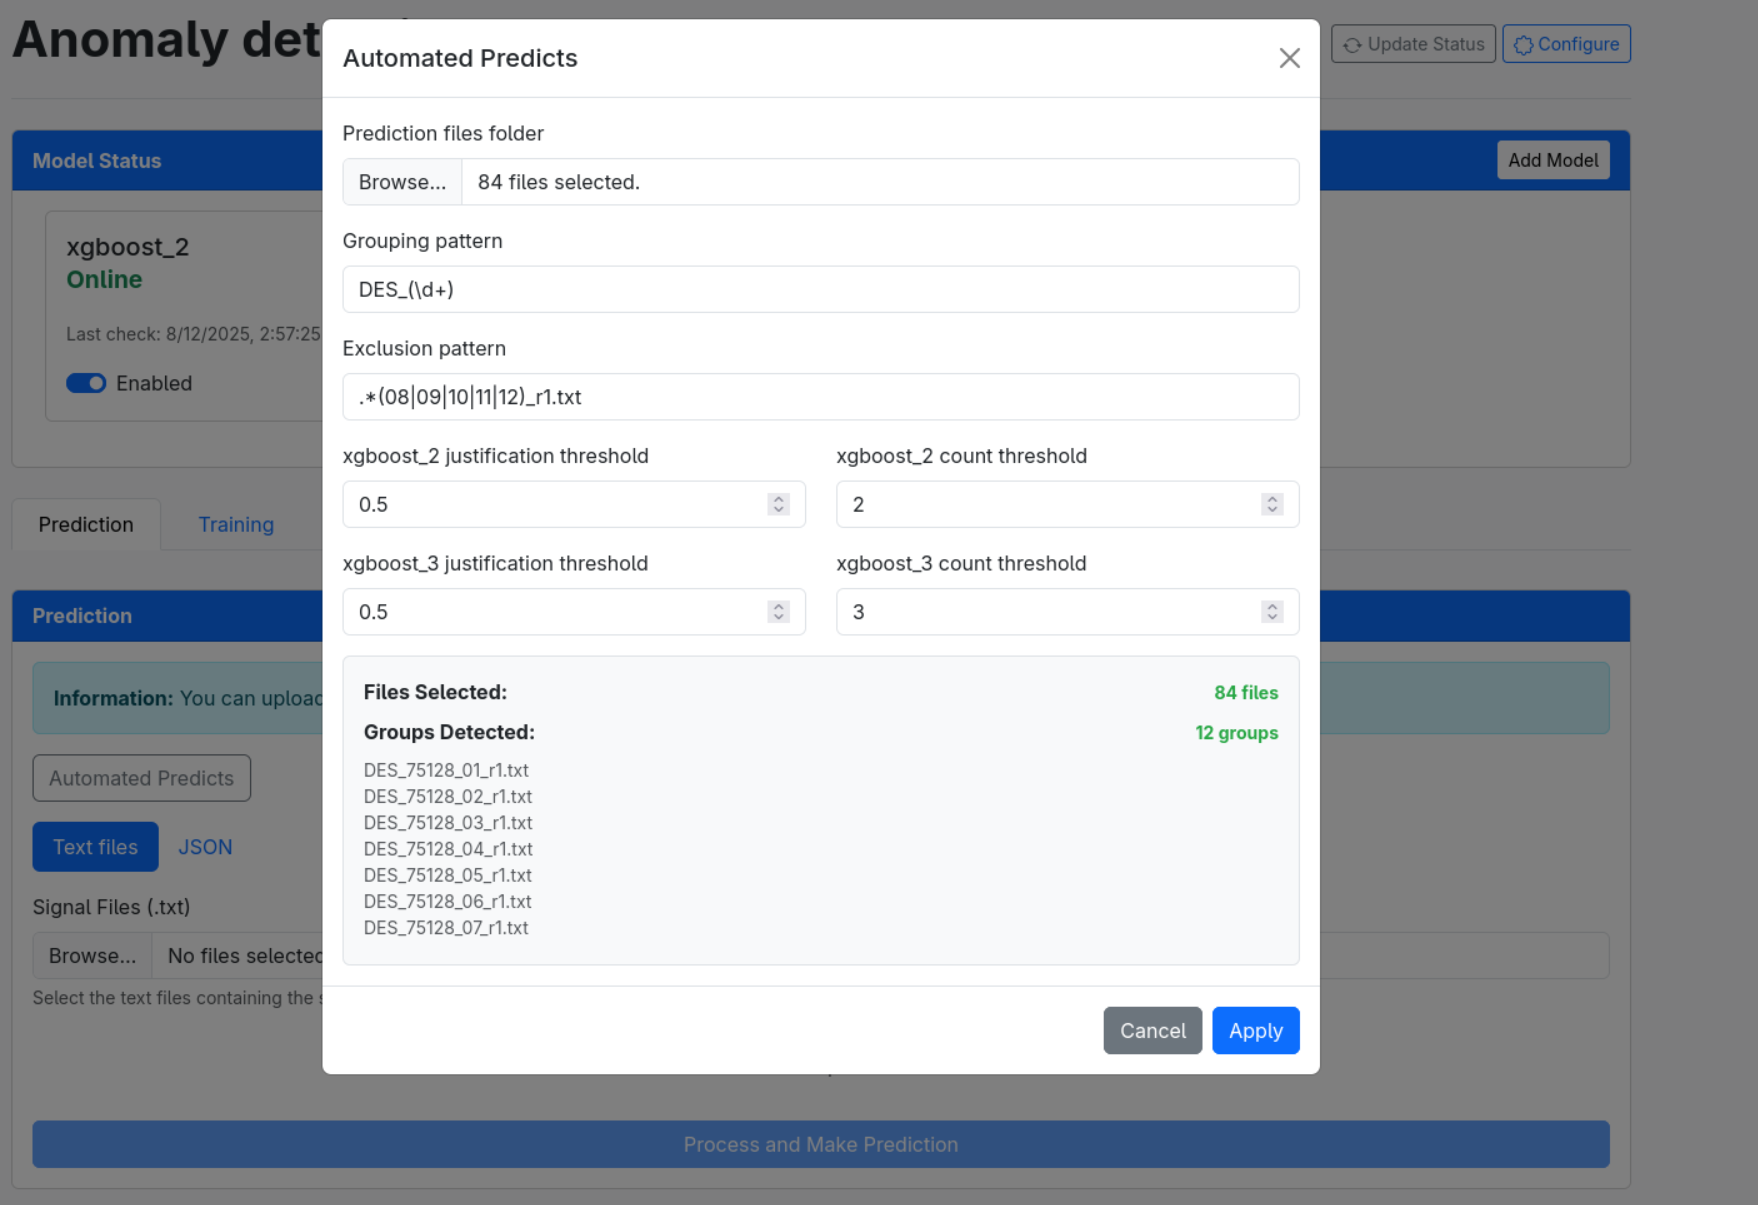
\includegraphics[width=\textwidth]{results/xgboost.png}
    \caption{XGBoost configuration}
    \label{fig:xgboost-config}
\end{figure}

\subsubsection{Non-disruptive discharges: 75223 and 75581}

Discharges 75223 and 75581 are non-disruptive. The plasma current signal is represented in blue for 75223 and orange for 75581 at \autoref{fig:ip_75223_75581}, compared with other similar C23 signals, used by the model to trigger anomaly alerts.\ \autoref{fig:xgboost-75223} shows both models predictions for discharge 75223, where the \texttt{xgboost\_2} alerts are represented in green, while the \texttt{xgboost\_3} alerts are in pink. There are also lines that reach the maximum value, and represent when the threshold has been reached. As can be seen, the \texttt{xgboost\_2} model triggers an alert around window 700, while the \texttt{xgboost\_3} model does not trigger any alert.\ \autoref{fig:xgboost-75581} shows the predictions for discharge 75581, where none of the models trigger an alert, as expected, since this is a non-disruptive discharge.

\begin{figure}[H]
    \centering
    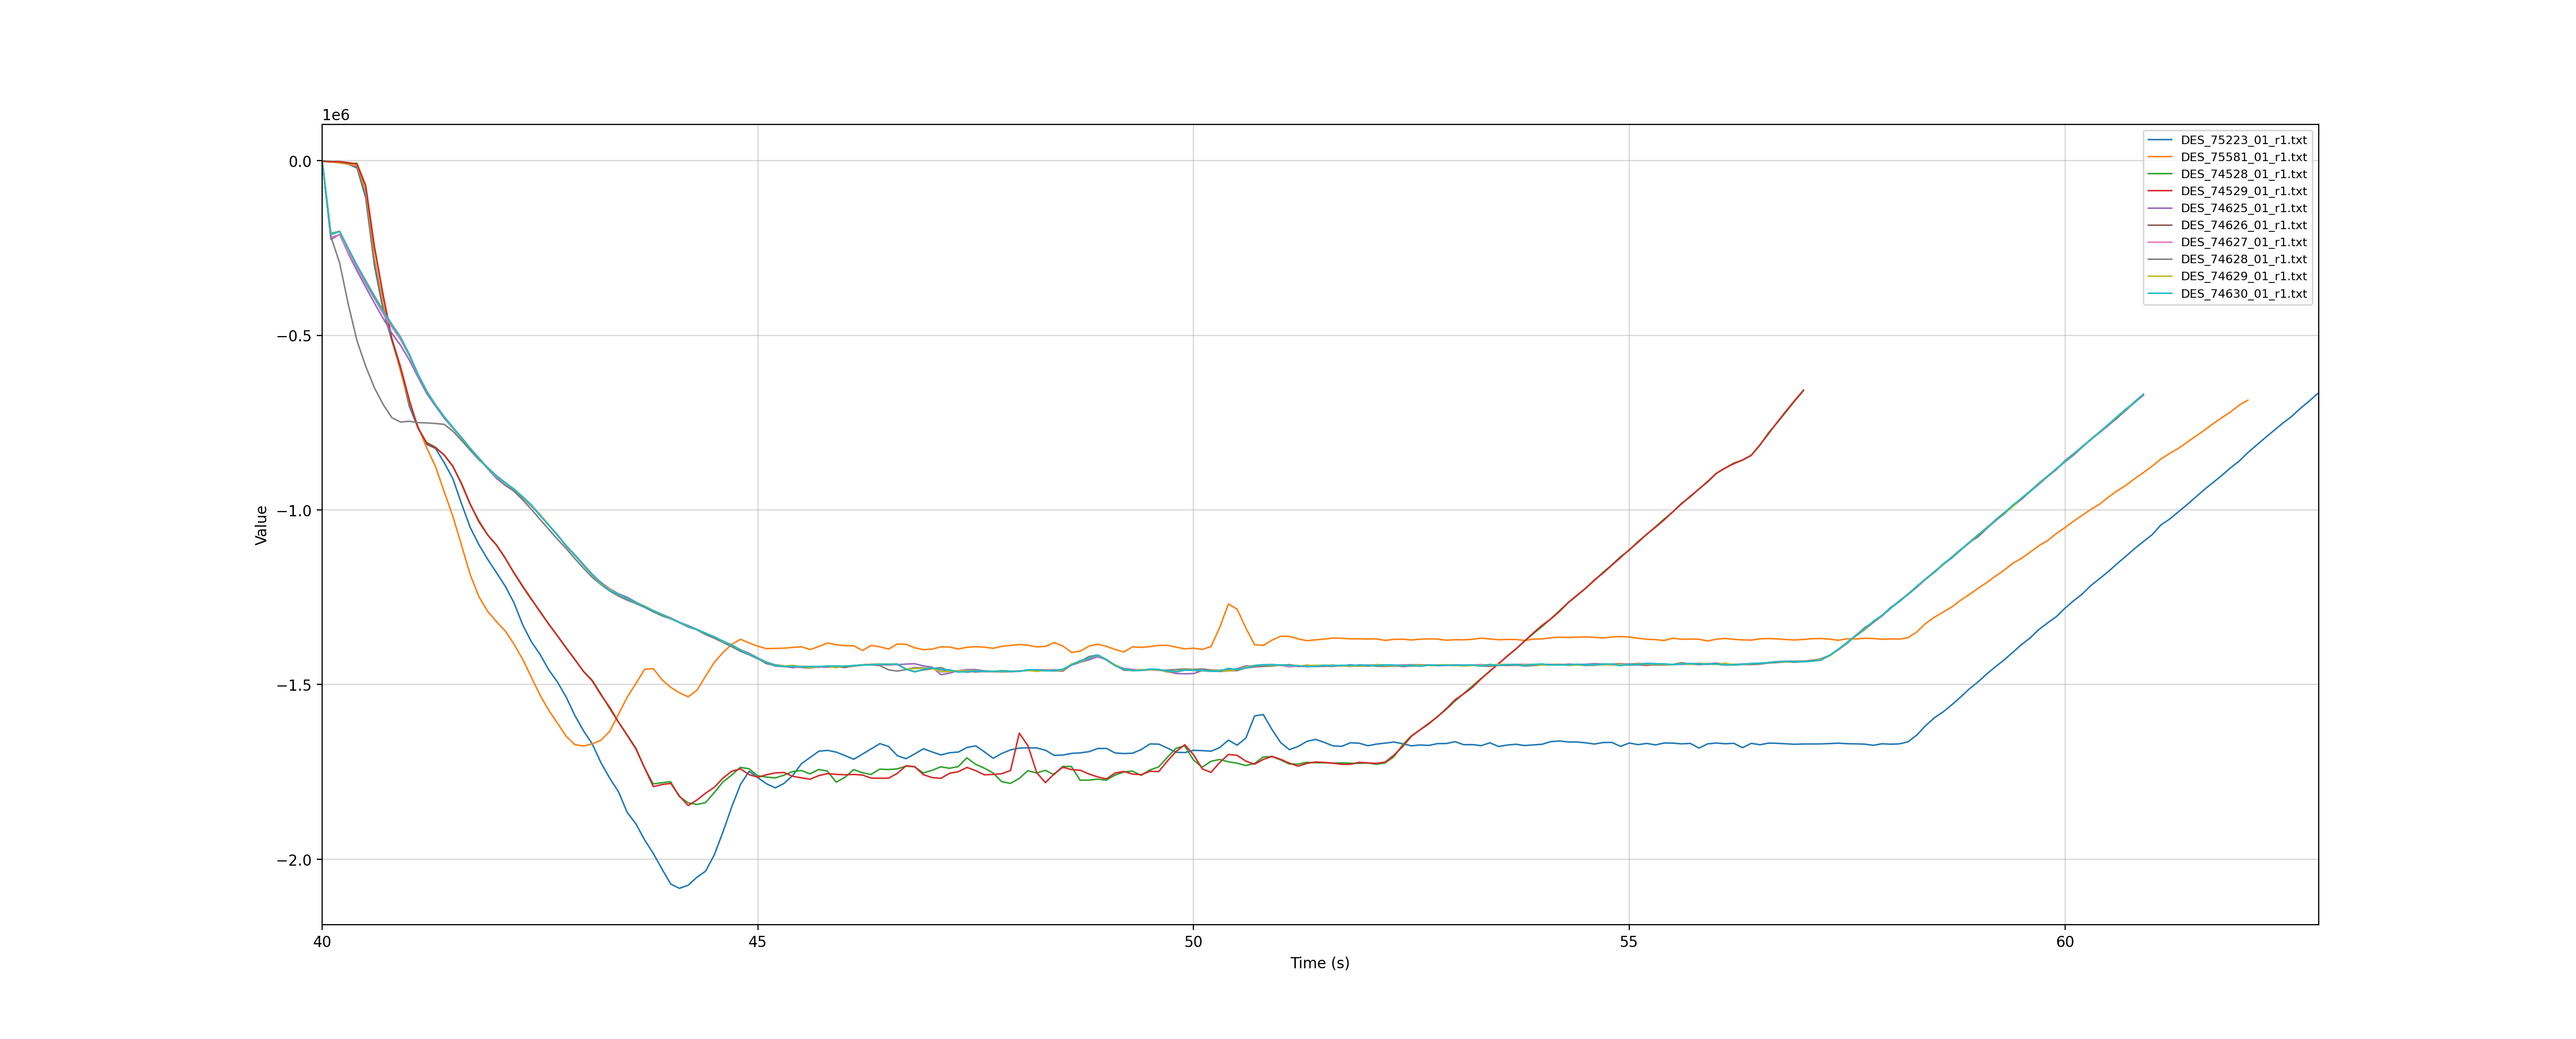
\includegraphics[width=\textwidth]{results/xgboost/75223_75581_vs_C23.png}
    \caption{Plasma current on discharges 75223 (blue) and 75581 (orange) compared to similar C23 non-disruptive discharges}
    \label{fig:ip_75223_75581}
\end{figure}

\begin{figure}[H]
    \centering
    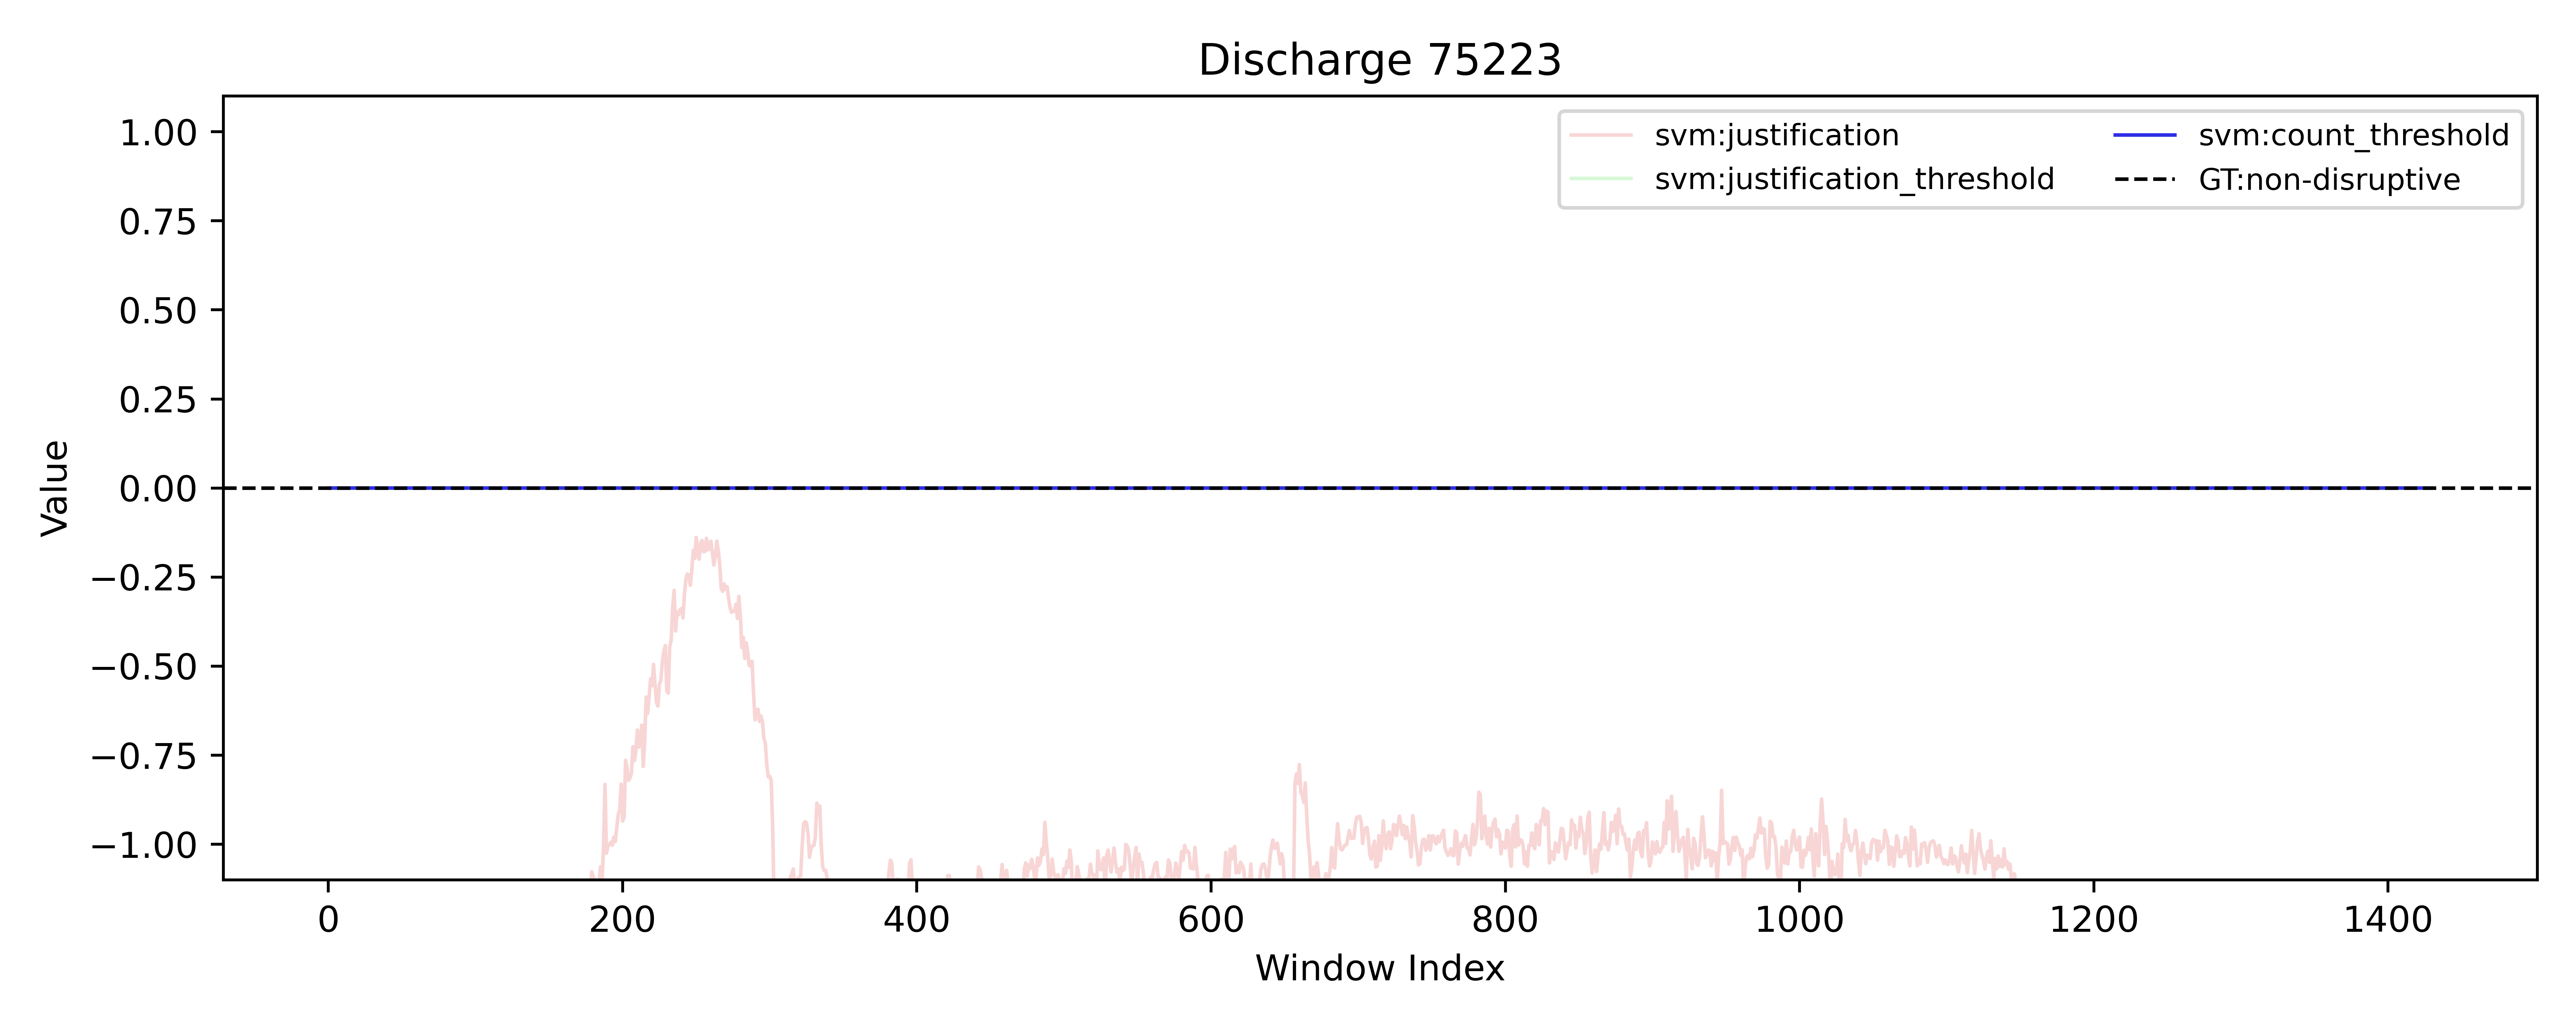
\includegraphics[width=\textwidth]{results/xgboost/75223.png}
    \caption{XGBoost prediction for discharge 75223}
    \label{fig:xgboost-75223}
\end{figure}

\begin{figure}[H]
    \centering
    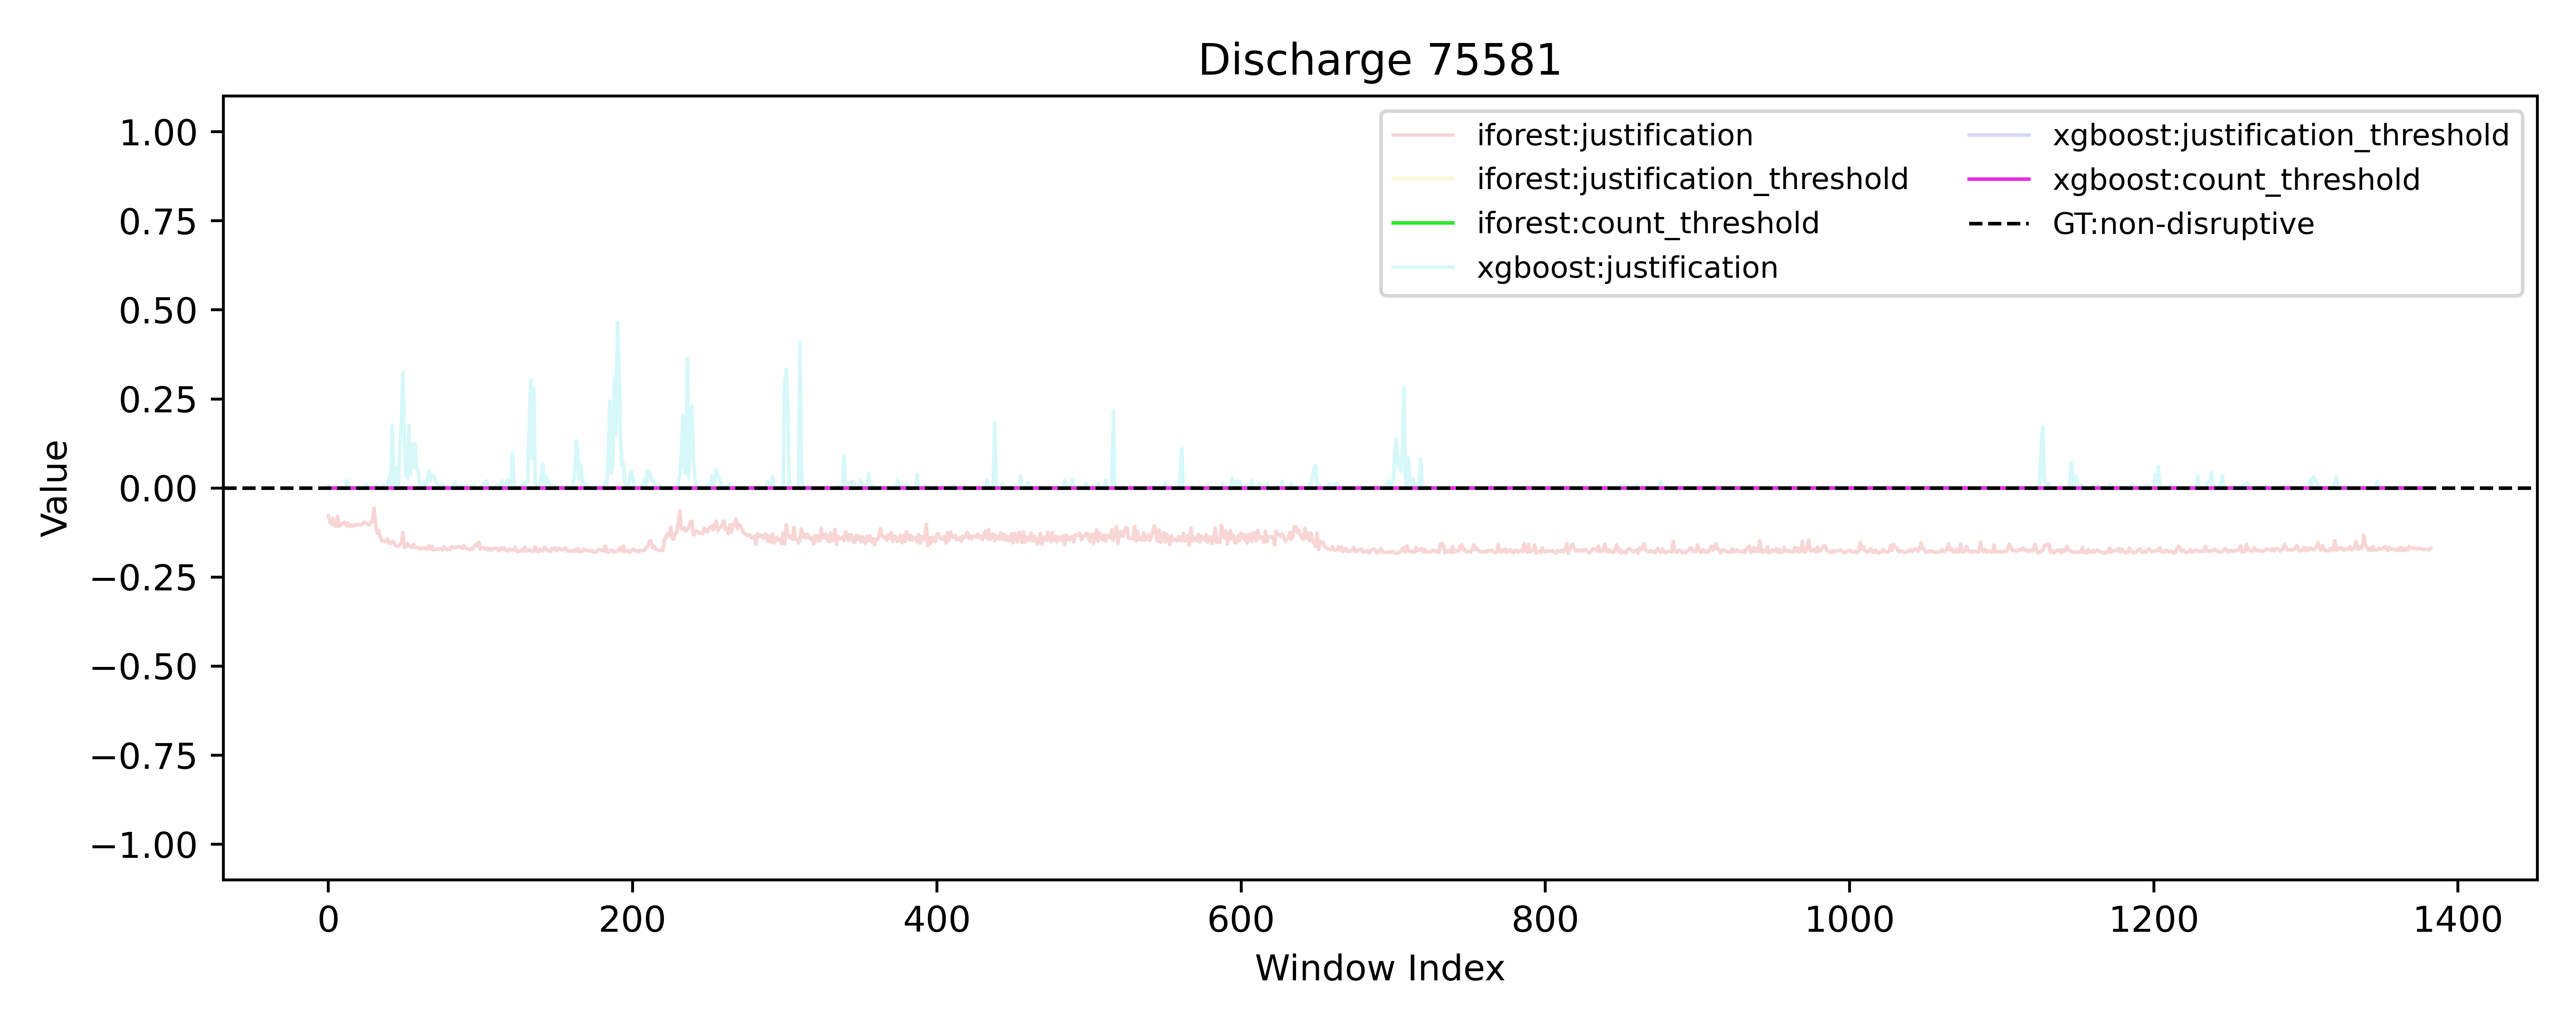
\includegraphics[width=\textwidth]{results/xgboost/75581.png}
    \caption{XGBoost prediction for discharge 75581}
    \label{fig:xgboost-75581}
\end{figure}

\subsubsection{Disruptive Discharges: 75273 and 75485}

Discharges 75273 and 75485 are disruptive discharges.\ \autoref{fig:ip_75273} and \autoref{fig:ip_75485} show the plasma current (in this case, in blue), compared with other similar C23 disruptive discharges.\ \autoref{fig:xgboost-75273} and \autoref{fig:xgboost-75485} show the predictions of both models for these discharges. In this case, both models trigger many alerts (\texttt{xgboost\_3} alerts are on top of \texttt{xgboost\_2} alerts), correctly identifying the discharges as anomalous.

\begin{figure}[H]
    \centering
    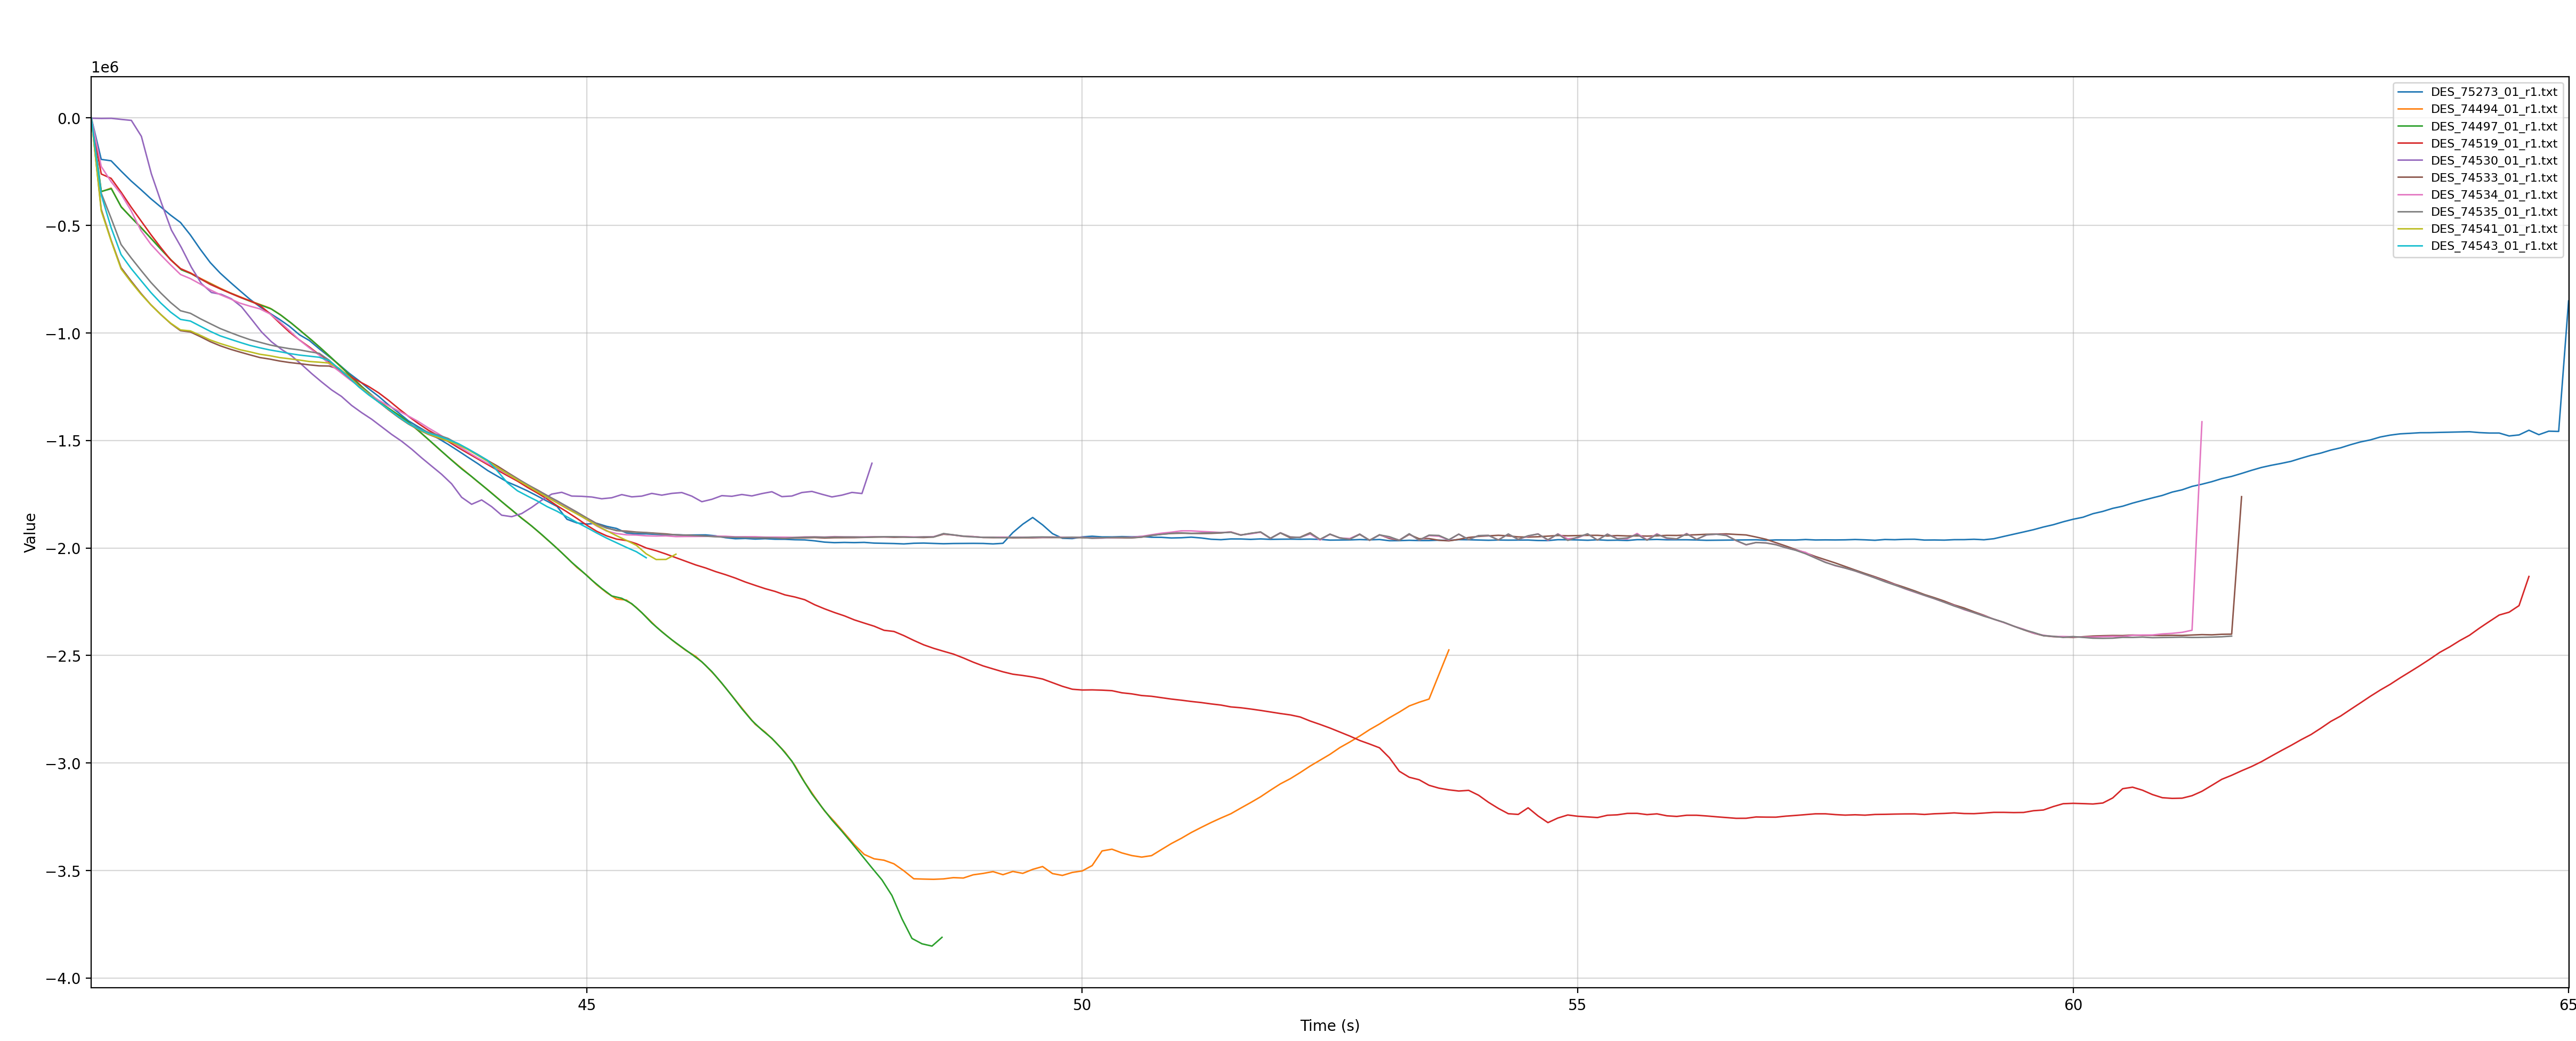
\includegraphics[width=\textwidth]{results/xgboost/75273_vs_C23.png}
    \caption{Plasma current on discharge 75273 (blue) compared to similar C23 disruptive discharges}
    \label{fig:ip_75273}
\end{figure}

\begin{figure}[H]
    \centering
    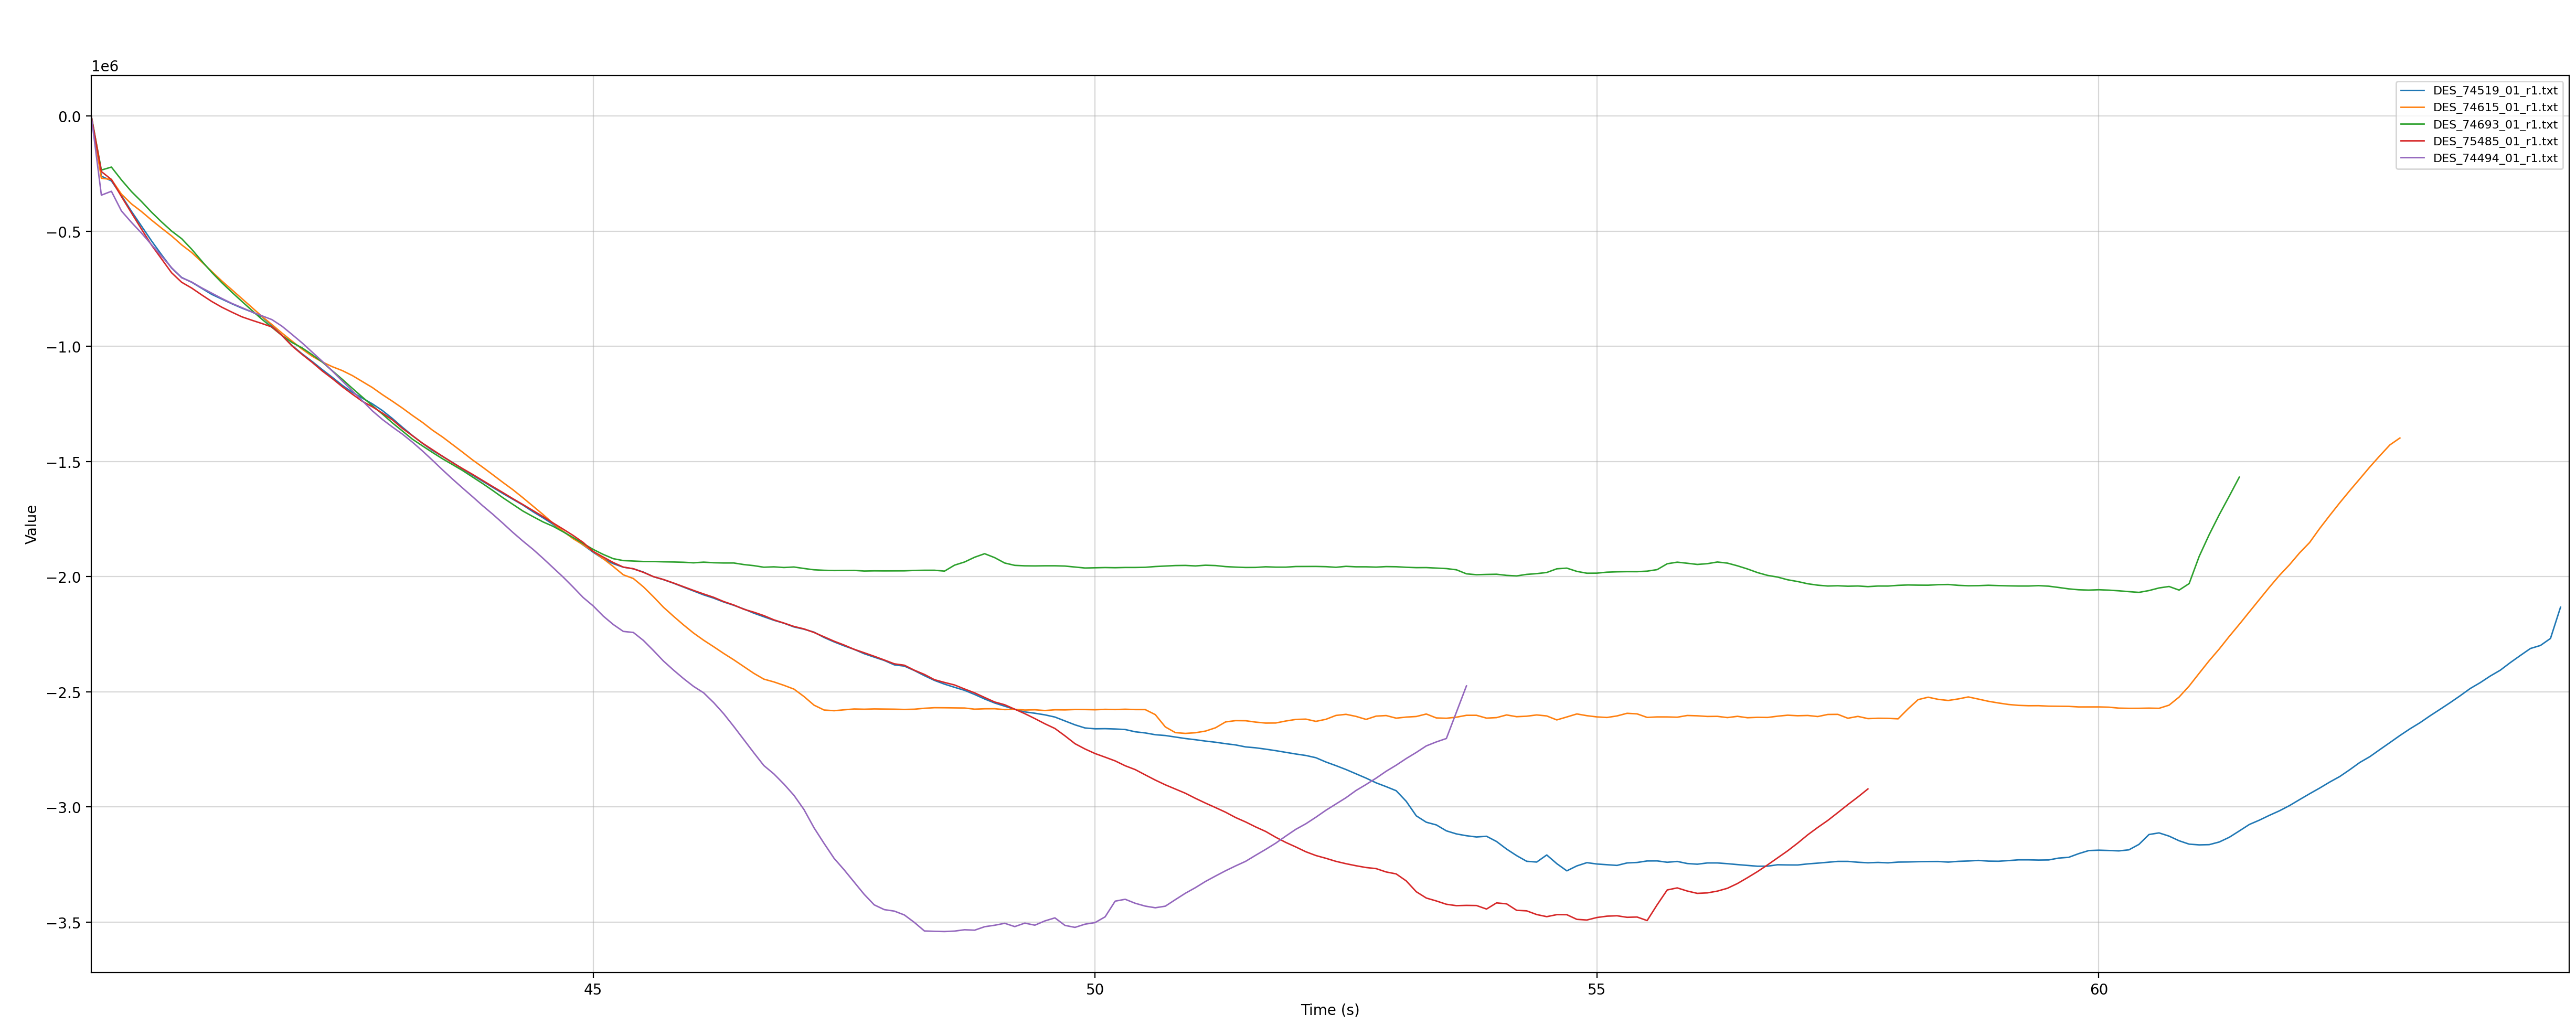
\includegraphics[width=\textwidth]{results/xgboost/75485_vs_C23.png}
    \caption{Plasma current on discharge 75485 (red) compared to similar C23 disruptive discharges}
    \label{fig:ip_75485}
\end{figure}

\begin{figure}[H]
    \centering
    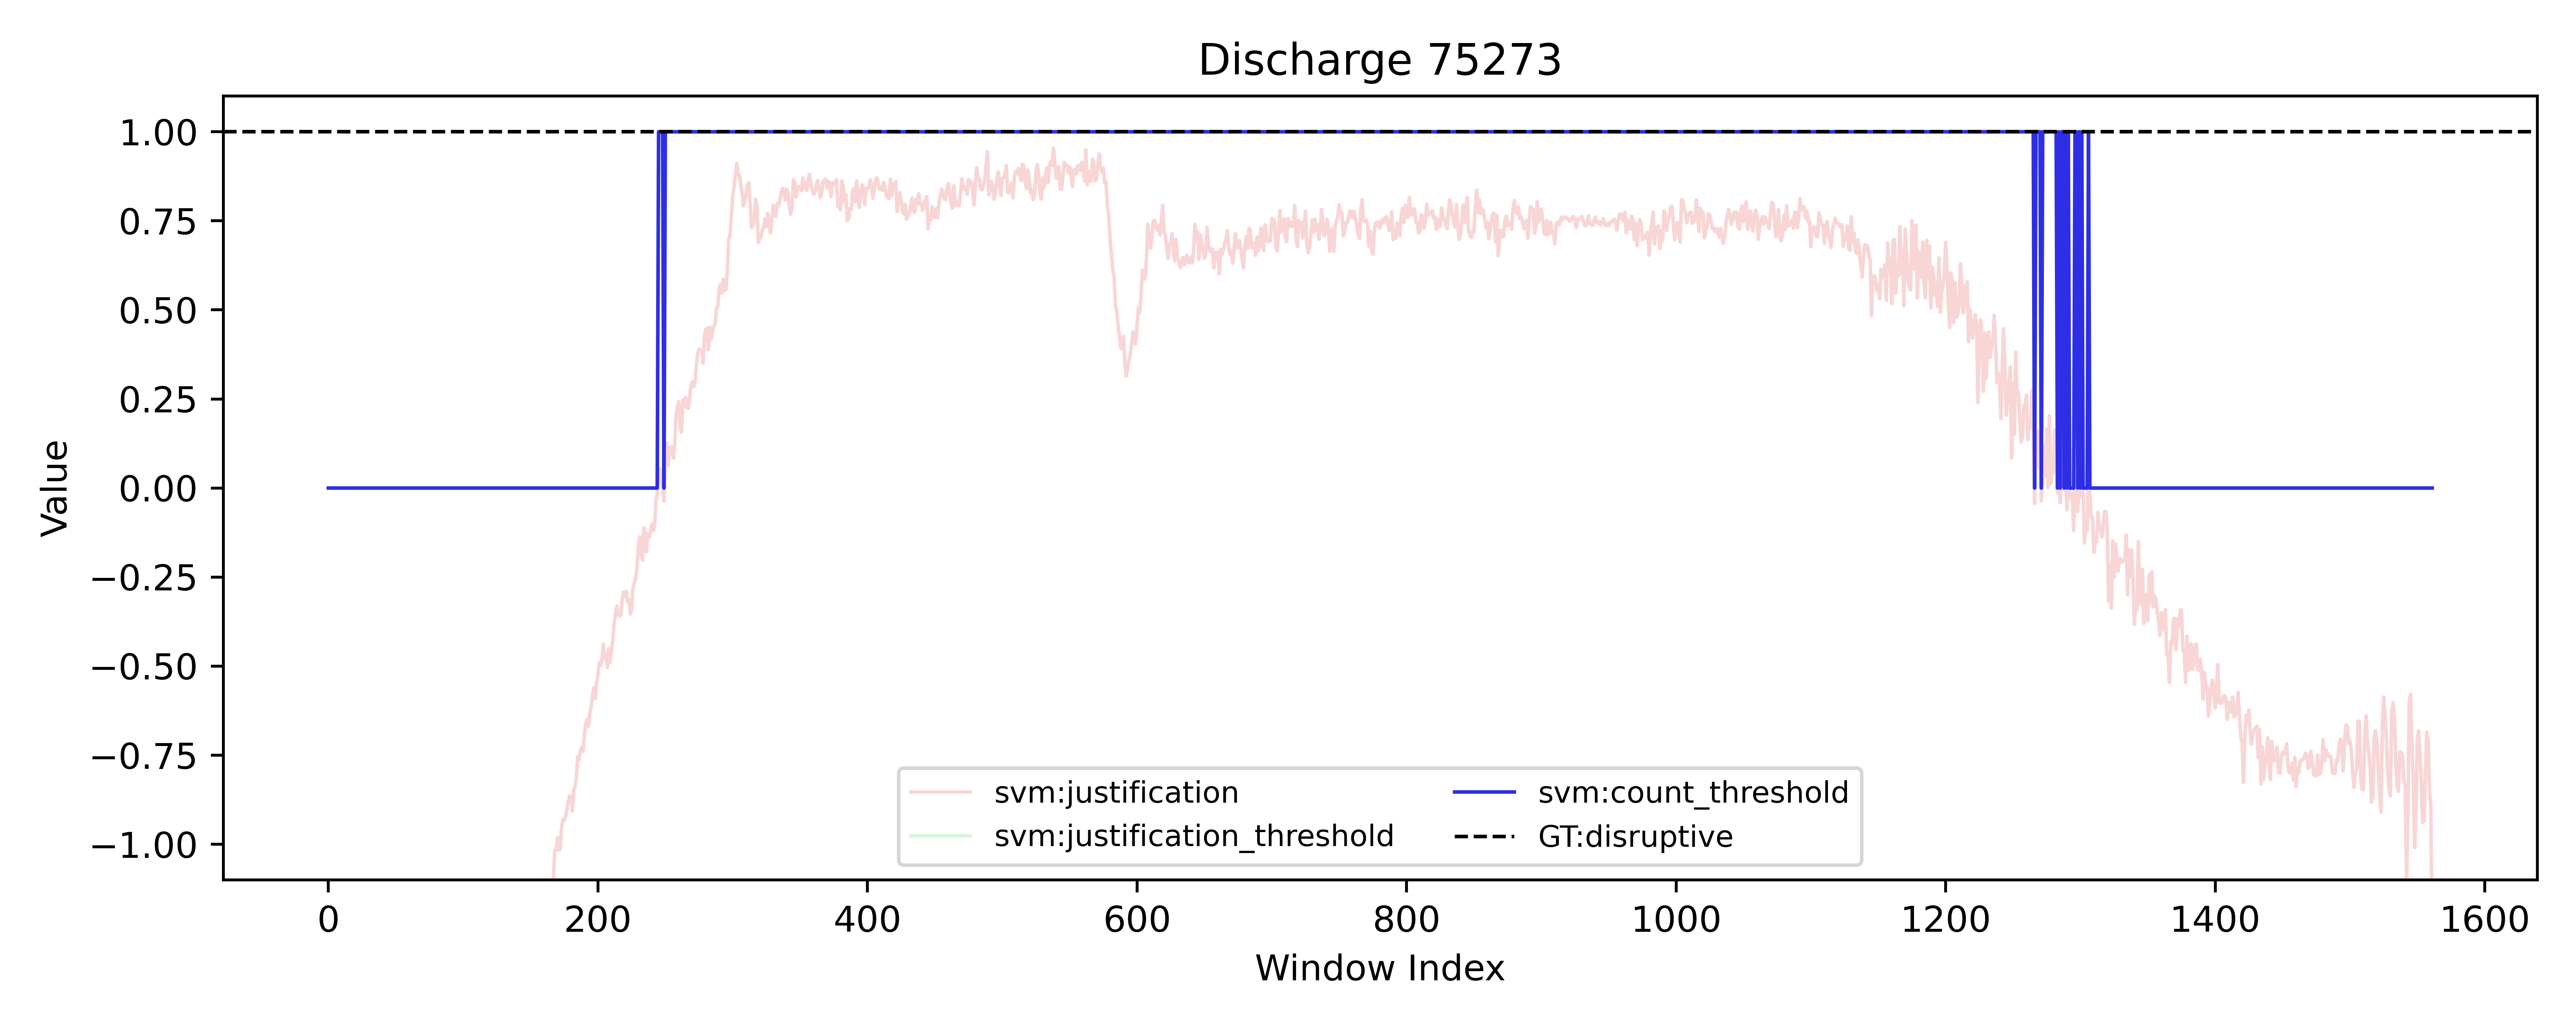
\includegraphics[width=\textwidth]{results/xgboost/75273.png}
    \caption{XGBoost prediction for discharge 75273}
    \label{fig:xgboost-75273}
\end{figure}

\begin{figure}[H]
    \centering
    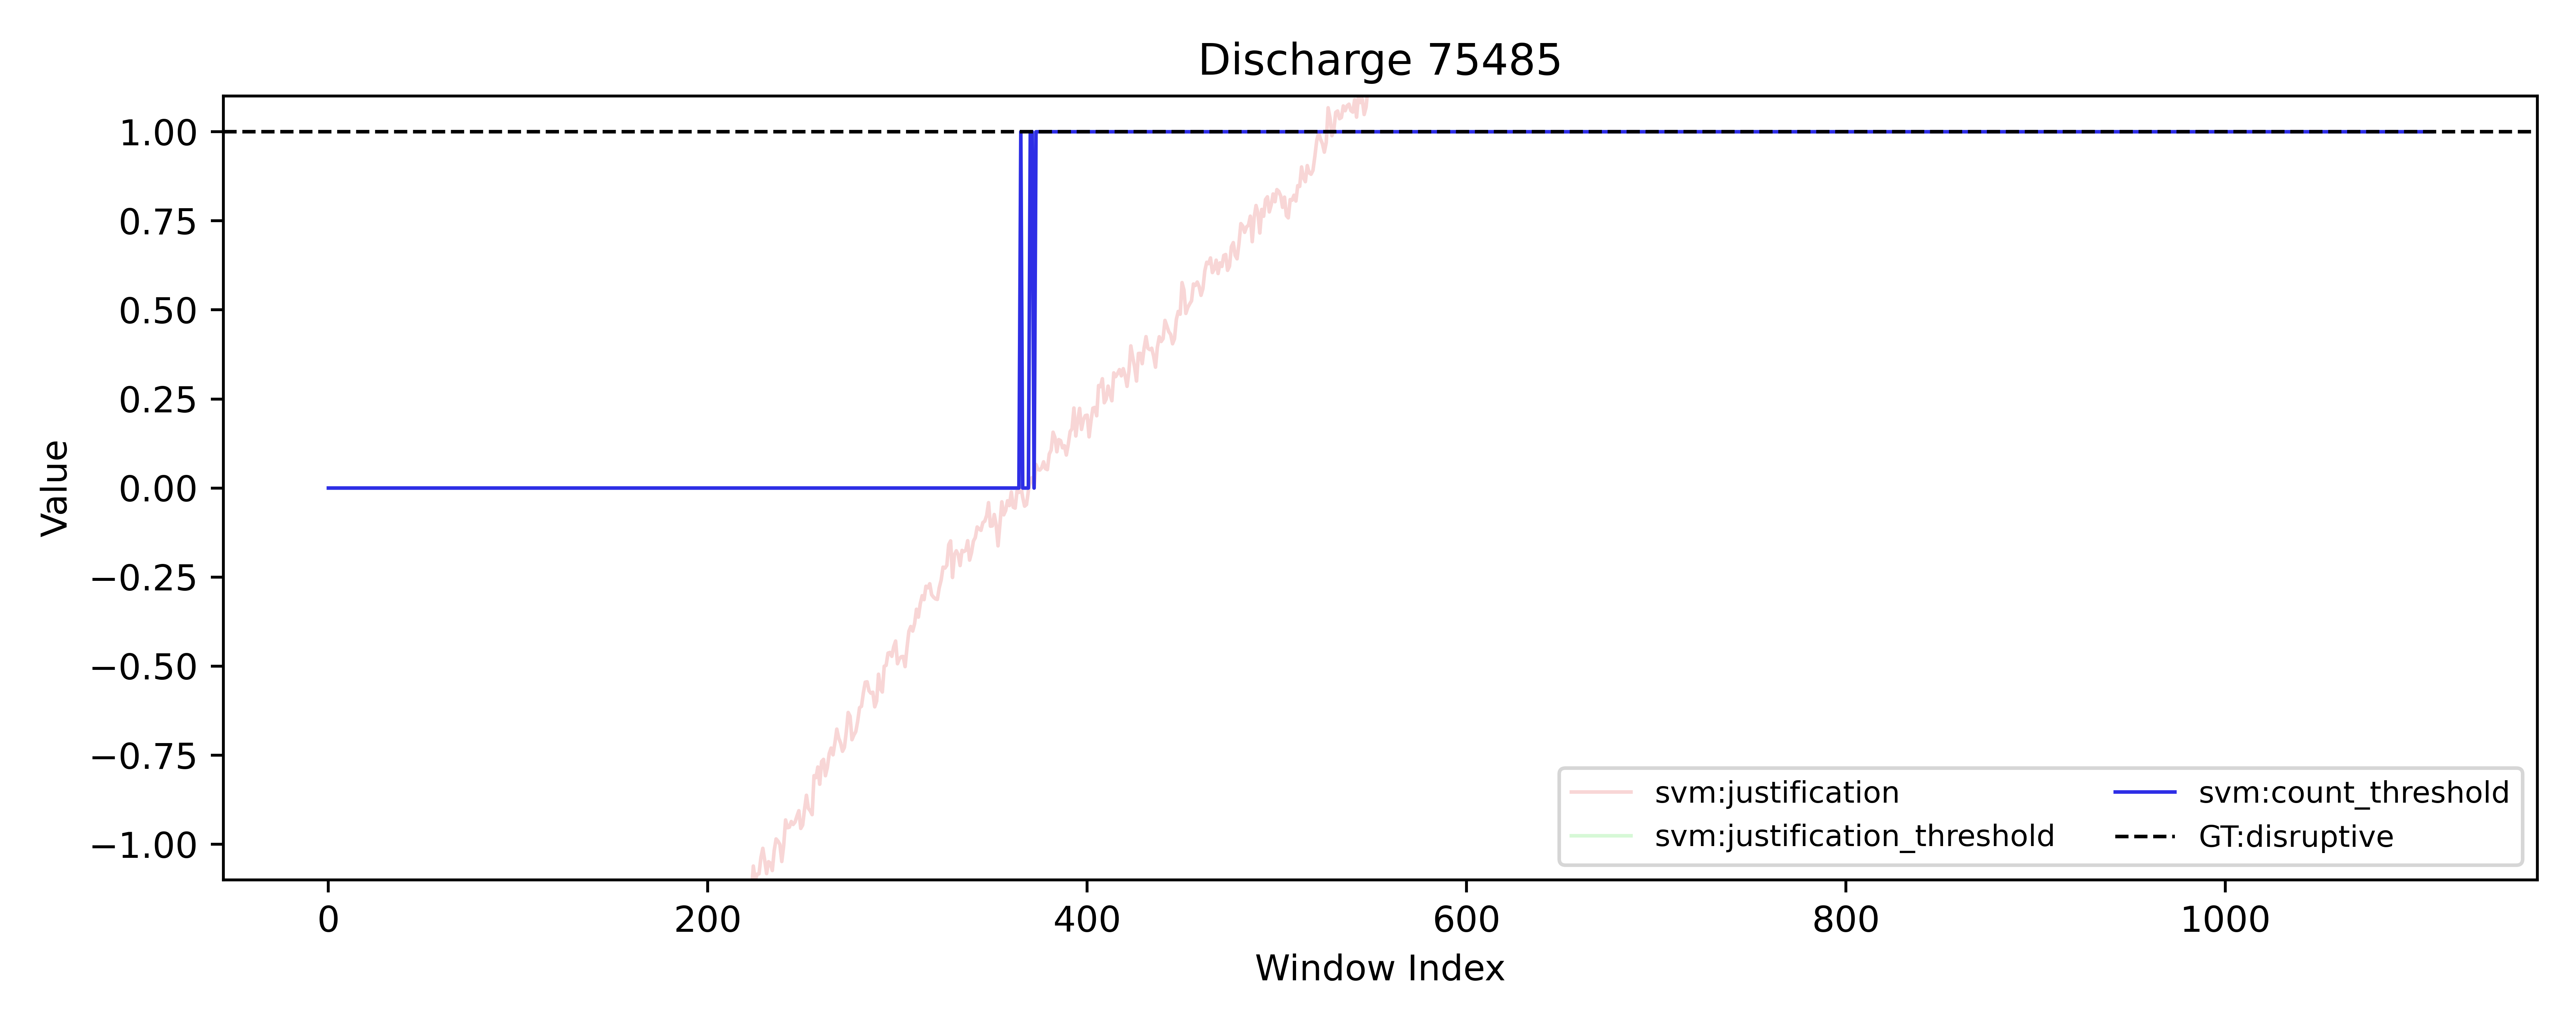
\includegraphics[width=\textwidth]{results/xgboost/75485.png}
    \caption{XGBoost prediction for discharge 75485}
    \label{fig:xgboost-75485}
\end{figure}

\subsubsection{False positives: 75128}

Discharge 75128 is a non-disruptive discharge, but \texttt{xgboost\_2} and \texttt{xgboost\_3} models trigger alerts, labeling this discharge as anomalous. This is caused because of the high correlation between this discharge and some of the disruptive discharges used for training the model, as shown in \autoref{fig:ip_75128}, where the plasma current of discharge 75128 (in blue) is compared with similar C23 disruptive discharges. Even though the discharge is also similar to some of non-disruptive discharges, weigh of the disruptive discharges is higher, as shown in \autoref{eq:gbdt-objective}, where $w_i$ is $\approx$ 11 times higher for disruptive discharges than for non-disruptive discharges, as this is the ratio of the number of disruptive windows to the number of non-disruptive windows in the training set. This leads to a model that is more sensitive to disruptive discharges, but also more prone to false positives when the discharge is similar to a disruptive discharge. 

\autoref{fig:xgboost-75128} shows the predictions of both models for discharge 75128.

\begin{figure}[H]
    \centering
    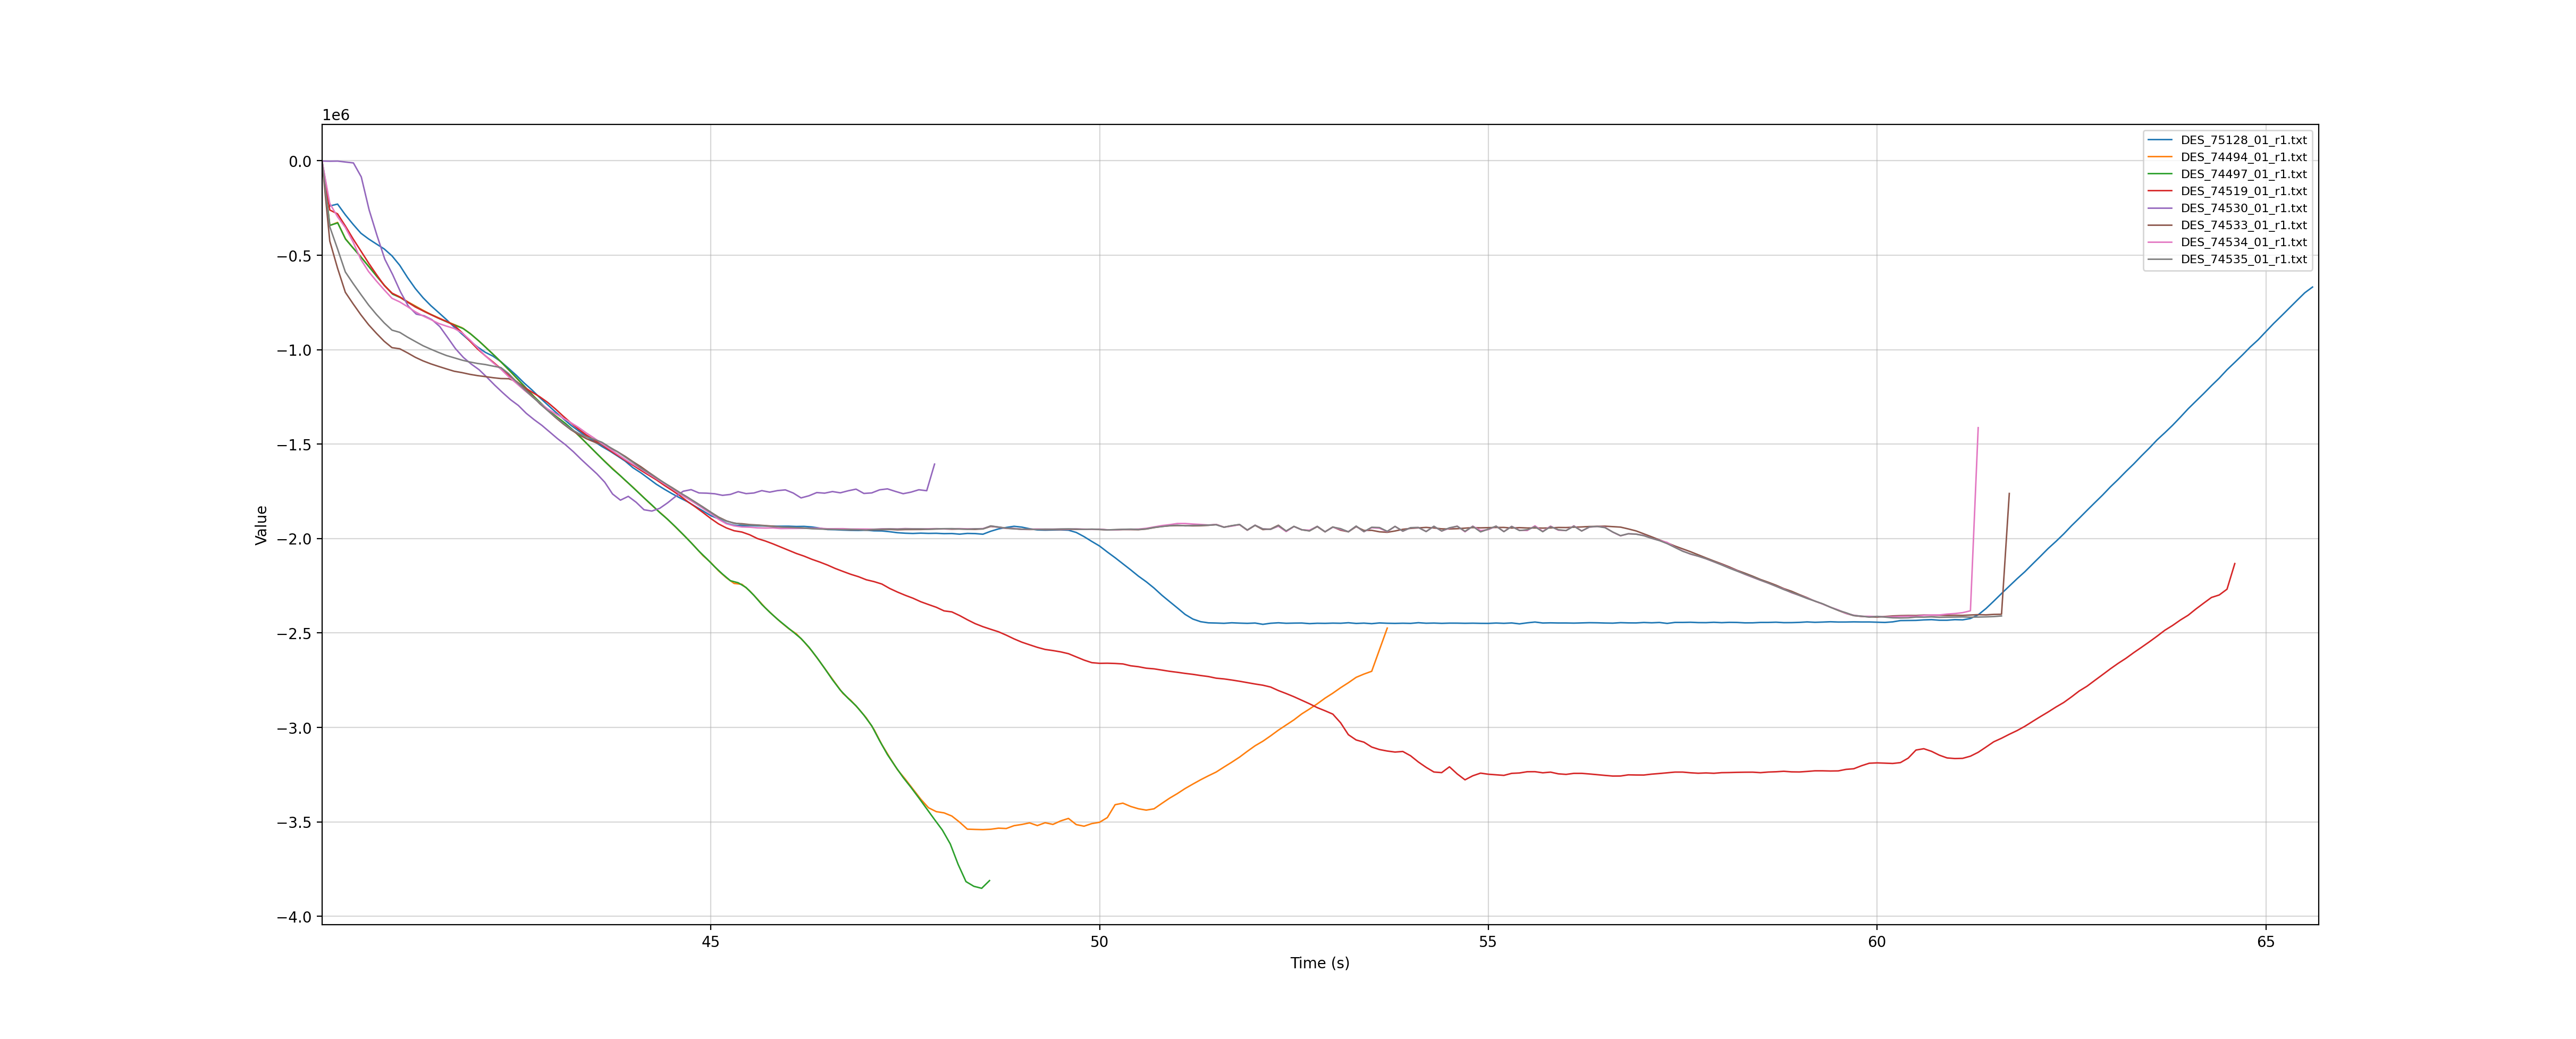
\includegraphics[width=\textwidth]{results/xgboost/75128_vs_C23.png}
    \caption{Plasma current on discharge 75128 (blue) compared to similar C23 disruptive discharges}
    \label{fig:ip_75128}
\end{figure}

\begin{figure}[H]
    \centering
    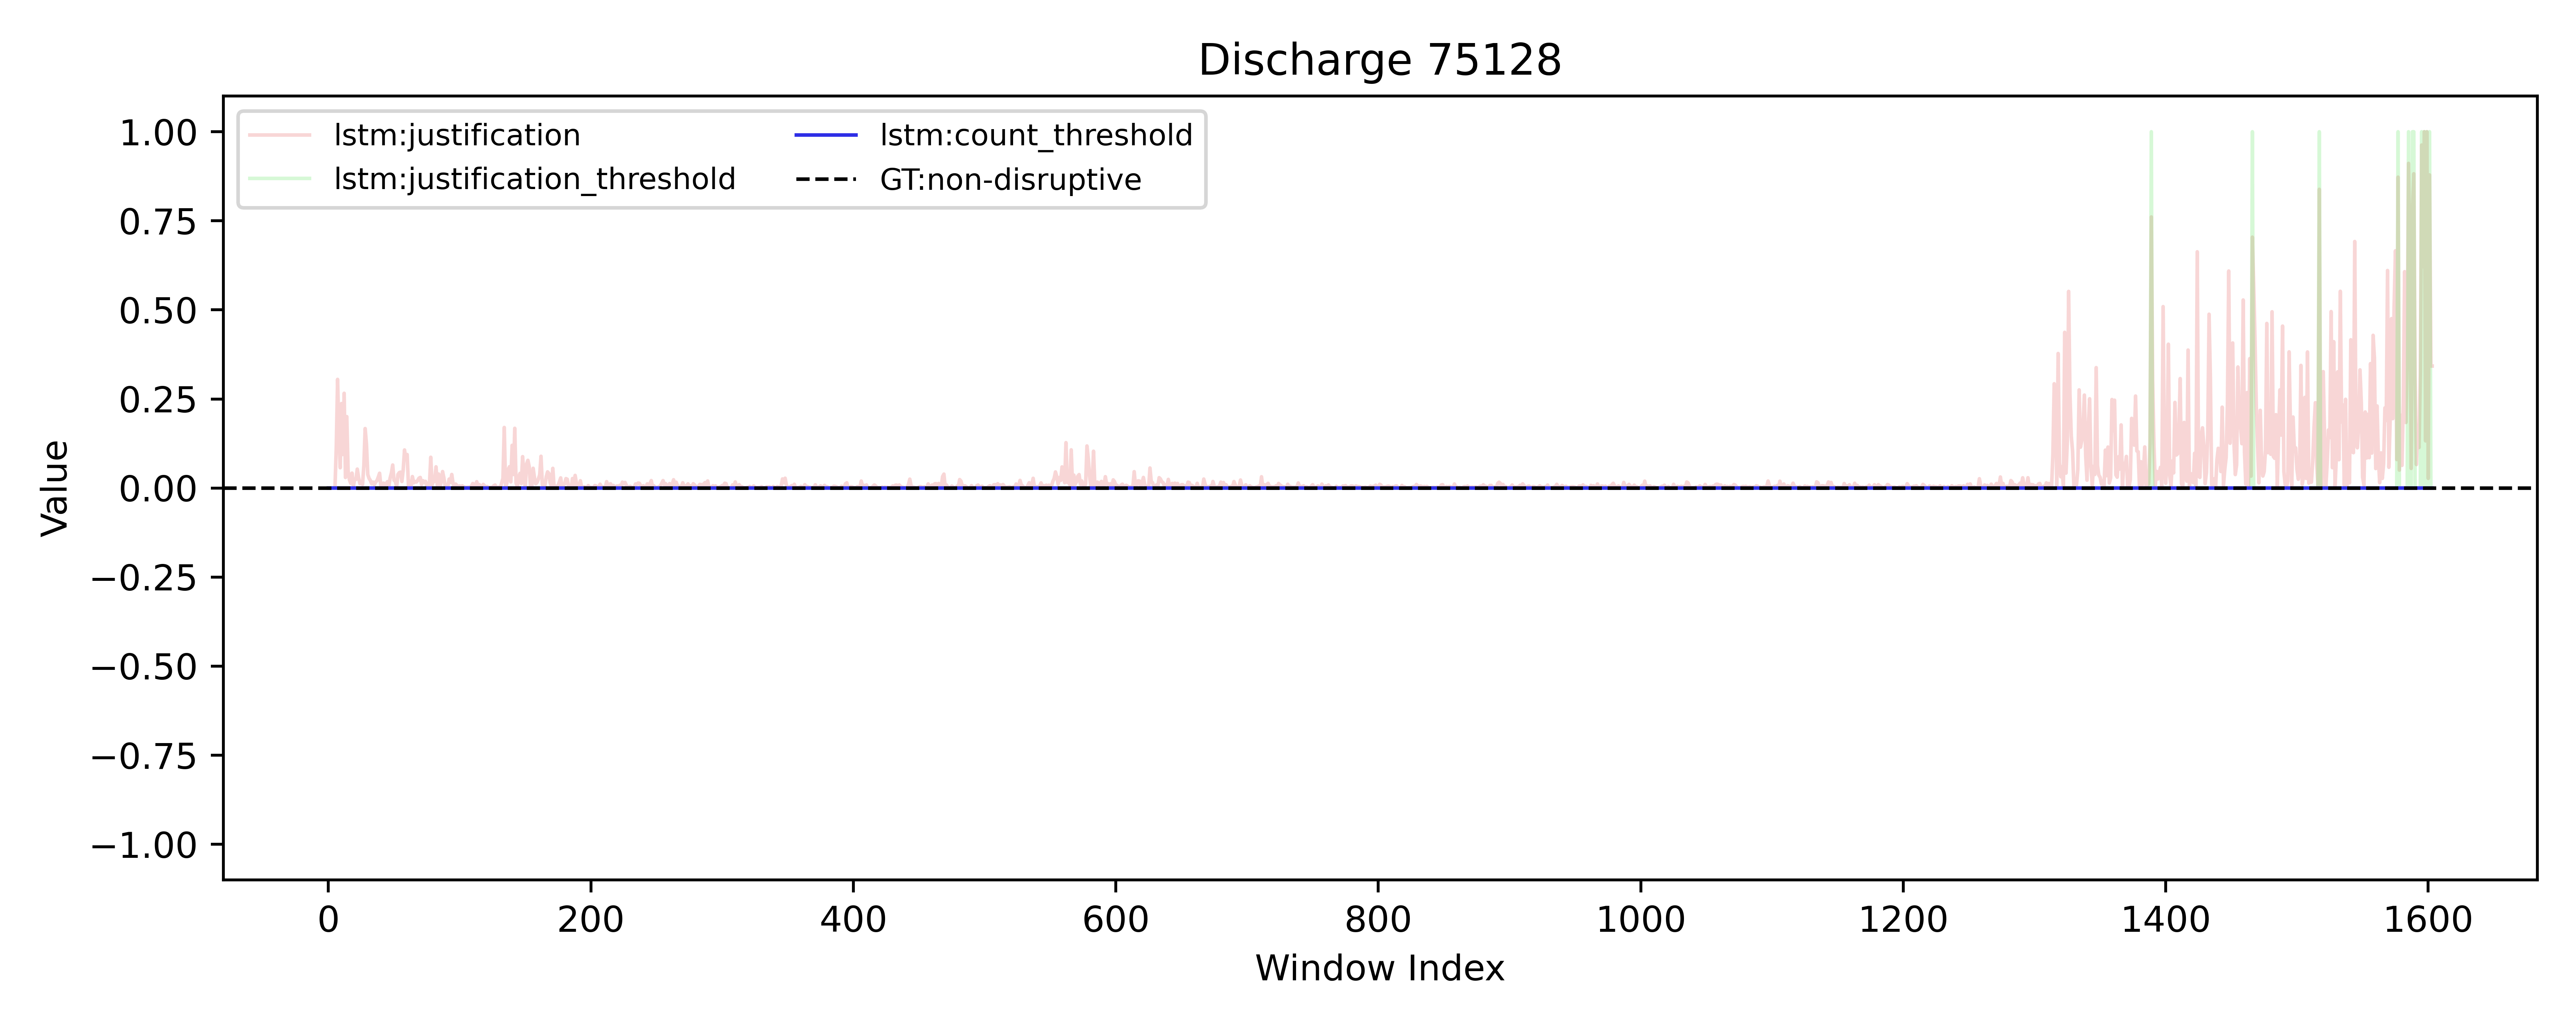
\includegraphics[width=\textwidth]{results/xgboost/75128.png}
    \caption{XGBoost prediction for discharge 75128}
    \label{fig:xgboost-75128}
\end{figure}



